% Provenance (never printed): see sources/outline_sources.md (Year 1: stress and
% principal stresses in 2D; strain; pure and simple shear; elastic, brittle and ductile
% behaviour; the strength envelope of the lithosphere). Strength envelopes from
% figdata/bachelor-1/strength_envelope.py (Byerlee 1975; flow laws of Gleason and Tullis
% 1995 and Hirth and Kohlstedt 2003 as compiled by Lopez-Sanchez; geotherms of ch. 10);
% exercise and problem values in the Book 3 scratch calculator calc/ch16.py. Traction,
% shear stress, the stress and strain tensors, Hooke's law, Young's modulus and viscosity
% belong to the physics series and are recalled, never defined (sync 1 ruling).
\chapter{Contrainte, déformation et rhéologie}\label{ch:b1:stress-strain-rheology}

Dans les années 1960, des eaux usées pompées dans un puits d'élimination au Rocky Mountain
Arsenal, près de Denver, se sont répandues dans le socle cristallin fracturé entre
\qty{3.7}{km} et \qty{7.0}{km} sous la surface, et des séismes ont suivi.
Ils sont restés dans la partie de la roche où la pression du fluide avait augmenté de
plus d'environ \qty{3.2}{MPa}.
% ledger: hb81:denver
Un demi-siècle plus tard la même chose s'est produite à plus grande échelle en Oklahoma,
où l'eau salée remontée avec le pétrole et le gaz est réinjectée dans le sous-sol. Dans
l'État et autour de lui, les séismes de magnitude 3 ou plus ont été au nombre de un à
cinq par an de 2005 à 2008, puis \num{20} en 2009, \num{585} en 2014 et
\num{888} en 2015, plus de deux par jour~; des secousses de magnitude 5.7 et 5.8 ont ébranlé
Prague, en 2011, et Pawnee, en 2016. Quatre puits d'élimination à fort débit à eux seuls
pourraient rendre compte d'un cinquième des séismes du centre des États-Unis, et
en ont déclenché certains à plus de \qty{30}{km}.
% ledger: usgs:oklahoma-rate, usgs:prague-pawnee, keranen:oklahoma
L'eau n'a rien repoussé~; elle a seulement élevé la pression
du fluide dans les pores de la roche. Pourquoi cela ferait-il glisser une faille~?
La réponse demande trois idées, qui sont le sujet de ce chapitre~: la
contrainte sur un plan à l'intérieur d'une roche, la condition dans laquelle le plan
cède, et le fait que la pression du fluide interstitiel s'oppose à la
force qui presse les deux côtés l'un contre l'autre. Avec elles, et avec une loi de fluage pour
la roche chaude, nous pouvons tracer la résistance de toute la \omterm{def:b1:layered-earth:lithosphere}{lithosphère} en fonction de la profondeur.

\begin{recall}
Une force répartie sur une surface agit par sa force par unité d'aire, en pascals~;
la pression dans un fluide au repos croît avec la profondeur comme $\rho g z$ (livres de physique).
Un ressort, et un solide en petites déformations, obéissent à la loi de Hooke~: la déformation est
proportionnelle à la contrainte, avec le module d'Young pour constante~; un fluide
visqueux résiste en proportion de sa vitesse de cisaillement, avec sa viscosité pour
constante. Le volume de troisième année des livres de physique décrit contrainte et
déformation en trois dimensions avec des tenseurs~; ce chapitre n'en demande que deux. Une
matrice symétrique $2\times2$ a deux valeurs propres réelles et deux vecteurs propres
perpendiculaires (mathématiques, première année). Les \omterm{def:b1:heat-budget:geotherm}{géothermes} du
\cref{ch:b1:heat-budget} donnent la température en profondeur~; les failles ont été rencontrées au
livre~1, année~7.
\end{recall}

\section{La contrainte en deux dimensions}\label{sec:b1:stress-strain-rheology:stress}

Coupons une roche par la pensée le long d'une petite surface plane. La roche d'un côté presse
sur la roche de l'autre avec une force, et la force par unité d'aire est la
traction sur cette surface, dans le mot des livres de physique. Sa direction n'est pas, en
général, celle de la normale à la surface.

\begin{definition}[Contrainte normale]\label{def:b1:stress-strain-rheology:stress}
Sur un plan passant par un point d'une roche, la force par unité d'aire que la roche d'un
côté exerce sur l'autre a une composante selon la normale au plan,
la \emph{contrainte normale}\index{contrainte normale} $\sigma_n$, et une composante
le long du plan, la contrainte de cisaillement $\tau$. En sciences de la Terre la contrainte
normale est comptée positive quand elle comprime.
\end{definition}

La convention de signe est l'opposée de celle de l'ingénieur. Elle est choisie parce que
presque toute contrainte dans la Terre solide est une compression~: le poids de la
roche au-dessus presse sur tout ce qui est en dessous.

Nous travaillons dans un plan vertical, avec un axe $x$ horizontal et un axe $y$. Sur un
plan perpendiculaire à $x$ la \omterm{def:b1:stress-strain-rheology:stress}{contrainte normale} est $\sigma_{xx}$ et la contrainte de
cisaillement $\sigma_{xy}$~; sur un plan perpendiculaire à $y$ ce sont $\sigma_{yy}$
et $\sigma_{yx}$. Les deux contraintes de cisaillement sont égales~: sur un petit carré, les
forces de cisaillement sur les côtés verticaux font un couple de moment
$\sigma_{xy}a\cdot a$ pour un côté $a$, celles sur les côtés horizontaux un couple
$\sigma_{yx}a\cdot a$ tournant dans l'autre sens, et le carré tournerait sur lui-même s'ils
différaient. Donc trois nombres décrivent la contrainte en un point, et ils
suffisent à la donner sur tout plan.

\begin{proposition}[Contrainte sur un plan incliné]\label{prop:b1:stress-strain-rheology:transformation}
Soit un plan de normale unitaire $\vec n = (\cos\theta, \sin\theta)$, à
l'angle $\theta$ de l'axe $x$, et soit $\vec m = (-\sin\theta, \cos\theta)$
le vecteur unitaire le long du plan. Les \omterm{def:b1:stress-strain-rheology:stress}{contraintes normale} et de cisaillement sur lui sont
\begin{align*}
  \sigma_n &= \sigma_{xx}\cos^2\theta + 2\sigma_{xy}\sin\theta\cos\theta + \sigma_{yy}\sin^2\theta
           = \frac{\sigma_{xx}+\sigma_{yy}}{2} + \frac{\sigma_{xx}-\sigma_{yy}}{2}\cos2\theta + \sigma_{xy}\sin2\theta, \\
  \tau     &= (\sigma_{yy}-\sigma_{xx})\sin\theta\cos\theta + \sigma_{xy}(\cos^2\theta - \sin^2\theta)
           = -\frac{\sigma_{xx}-\sigma_{yy}}{2}\sin2\theta + \sigma_{xy}\cos2\theta ,
\end{align*}
avec $\tau$ compté positivement selon $\vec m$.
\end{proposition}

\begin{proof}
Découpons un petit prisme, comme sur la figure ci-dessous~: une
face inclinée d'aire $A$ de normale sortante $\vec n$, une face verticale
d'aire $A\cos\theta$ et une face horizontale d'aire $A\sin\theta$, par unité de
longueur dans la troisième direction. Son poids et son inertie varient comme son volume,
qui diminue plus vite que ses faces~; pour un prisme assez petit les forces sur
les faces doivent s'équilibrer à elles seules. La compression étant positive, la roche
extérieure pousse sur la face verticale avec la force
$A\cos\theta\,(\sigma_{xx}, \sigma_{xy})$ et sur la face horizontale avec
$A\sin\theta\,(\sigma_{xy}, \sigma_{yy})$~; sur la face inclinée elle pousse
avec $-A(\sigma_n\vec n + \tau\vec m)$. La somme est nulle~:
\[
  \sigma_n\vec n + \tau\vec m = \cos\theta\,(\sigma_{xx}, \sigma_{xy}) + \sin\theta\,(\sigma_{xy}, \sigma_{yy}) .
\]
Le produit scalaire avec $\vec n$ donne $\sigma_n$, avec $\vec m$ donne $\tau$,
puisque $\vec n\cdot\vec m = 0$. Les secondes formes découlent de
$\cos^2\theta = (1+\cos2\theta)/2$, $\sin^2\theta = (1-\cos2\theta)/2$ et
$2\sin\theta\cos\theta = \sin2\theta$.
\end{proof}

\begin{omfigure}
\begin{tikzpicture}[>={Stealth[length=5pt]}, font=\small]
% theta = 35 deg, hypotenuse L = 4.5: a = L cos(theta), b = L sin(theta)
\pgfmathsetmacro{\th}{35}
\pgfmathsetmacro{\L}{4.5}
\pgfmathsetmacro{\a}{\L*cos(\th)}
\pgfmathsetmacro{\b}{\L*sin(\th)}
\coordinate (O) at (0,0);
\coordinate (A) at (0,\a);
\coordinate (B) at (\b,0);
\coordinate (M) at ($(A)!0.5!(B)$);
\fill[omLithGranite!45] (O) -- (A) -- (B) -- cycle;
\draw[line width=0.8pt] (O) -- (A) -- (B) -- cycle;
% axes
\draw[->, black!70] (-2.6,-1.9) -- (-1.6,-1.9) node[right] {$x$};
\draw[->, black!70] (-2.6,-1.9) -- (-2.6,-0.9) node[above] {$y$};
% face on x = 0 (outward normal -x), area A cos(theta)
\draw[->, line width=1.1pt, omDef] (-1.35,0.5*\a) -- (-0.05,0.5*\a);
\node[omDef, anchor=south] at (-0.95,0.5*\a+0.05) {$\sigma_{xx} A\cos\theta$};
\draw[->, line width=1.1pt, omProp] (-0.25,0.5*\a-1.25) -- (-0.25,0.5*\a-0.25);
\node[omProp, anchor=east] at (-0.3,0.5*\a-0.85) {$\sigma_{xy} A\cos\theta$};
% face on y = 0 (outward normal -y), area A sin(theta)
\draw[->, line width=1.1pt, omDef] (0.68*\b,-1.35) -- (0.68*\b,-0.05);
\node[omDef, anchor=west] at (0.68*\b+0.05,-1.05) {$\sigma_{yy} A\sin\theta$};
\draw[->, line width=1.1pt, omProp] (0.1,-0.25) -- (1.1,-0.25);
\node[omProp, anchor=north east] at (0.9,-0.32) {$\sigma_{xy} A\sin\theta$};
% inclined face, area A, normal n = (cos theta, sin theta)
\draw[->, line width=1.1pt, omThm] ($(M)+(\th:1.5)$) -- ($(M)+(\th:0.05)$);
\node[omThm, anchor=south west, inner sep=1pt] at ($(M)+(\th:1.5)$) {$\sigma_n A$};
\draw[->, line width=1.1pt, omThm!70!black] ($(M)+(\th:0.25)+(\th-90:0.75)$) -- ($(M)+(\th:0.25)+(\th-90:1.75)$);
\node[omThm!70!black, anchor=west] at ($(M)+(\th:0.3)+(\th-90:1.3)$) {$\tau A$};
\draw[->, black!70, dashed] ($(M)+(\th+90:1.25)$) -- ++(\th:1.0) node[pos=1, anchor=south west, inner sep=1pt, text=black] {$\boldsymbol n$};
% angle theta at A, between the face and the y axis
\pic[draw, angle radius=0.75cm, pic text={$\theta$}, angle eccentricity=1.35] {angle = O--A--B};
\end{tikzpicture}
\par\smallskip{\small L'équilibre des forces sur un petit prisme triangulaire de
roche. La face inclinée a l'aire $A$ et la normale unitaire $\vec n$~; les
faces verticale et horizontale ont les aires $A\cos\theta$ et $A\sin\theta$.
Bleu~: les forces normales sur les deux petites faces~; orange~: les forces de cisaillement sur
elles~; rouge~: les forces normale et de cisaillement sur la face inclinée. La compression est
comptée positive, donc chaque force normale pointe vers l'intérieur du prisme.}
\label{fig:b1:stress-strain-rheology:prism}
\end{omfigure}

\begin{theorem}[Contraintes principales]\label{thm:b1:stress-strain-rheology:principal}
En tout point d'une roche il y a deux plans perpendiculaires sur lesquels la contrainte de
cisaillement est nulle. Les \omterm{def:b1:stress-strain-rheology:stress}{contraintes normales} sur eux sont la plus grande et la plus petite
\omterm{def:b1:stress-strain-rheology:stress}{contrainte normale} sur tous les plans passant par le point,
\[
  \sigma_{1,3} = \frac{\sigma_{xx}+\sigma_{yy}}{2} \pm
  \sqrt{\Bigl(\frac{\sigma_{xx}-\sigma_{yy}}{2}\Bigr)^2 + \sigma_{xy}^2},
  \qquad \tan2\theta_p = \frac{2\sigma_{xy}}{\sigma_{xx}-\sigma_{yy}},
\]
où $\theta_p$ est l'angle de l'axe $x$ à la normale du plan
qui porte $\sigma_1$.
\end{theorem}

\begin{proof}
Posons $c = (\sigma_{xx}+\sigma_{yy})/2$, et choisissons $R \ge 0$ et $\theta_p$
avec $(\sigma_{xx}-\sigma_{yy})/2 = R\cos2\theta_p$ et
$\sigma_{xy} = R\sin2\theta_p$~; alors
$R = \sqrt{((\sigma_{xx}-\sigma_{yy})/2)^2 + \sigma_{xy}^2}$ et
$\tan2\theta_p$ est celui de l'énoncé. Les secondes formes de la
\cref{prop:b1:stress-strain-rheology:transformation} deviennent
\[
  \sigma_n = c + R\cos(2\theta - 2\theta_p), \qquad \tau = -R\sin(2\theta - 2\theta_p).
\]
La \omterm{def:b1:stress-strain-rheology:stress}{contrainte normale} est maximale, $c + R$, pour $\theta = \theta_p$, et minimale,
$c - R$, pour $\theta = \theta_p + \ang{90}$~; dans les deux cas, $\tau = 0$. Notons aussi
que $\mathrm d\sigma_n/\mathrm d\theta = 2\tau$~: la \omterm{def:b1:stress-strain-rheology:stress}{contrainte normale} est
stationnaire exactement là où la contrainte de cisaillement s'annule.
\end{proof}

\begin{definition}[Contraintes principales, contrainte différentielle]\label{def:b1:stress-strain-rheology:principal}
Les \emph{contraintes principales}\index{contraintes principales} en un point sont les
\omterm{def:b1:stress-strain-rheology:stress}{contraintes normales} $\sigma_1 \ge \sigma_3$ sur les deux plans sans contrainte de
cisaillement, et leurs directions sont les directions principales. En trois
dimensions il y en a trois, $\sigma_1 \ge \sigma_2 \ge \sigma_3$, sur trois
plans perpendiculaires. La \emph{contrainte différentielle}\index{contrainte differentielle@contrainte différentielle} est
$\sigma_1 - \sigma_3$, et la contrainte moyenne dans le plan est
$(\sigma_1+\sigma_3)/2$.
\end{definition}

Un état de contrainte se lit le plus facilement dans ses directions principales. Si l'on
mesure l'angle $\theta$ à partir de la direction de $\sigma_1$ et non à partir de
l'axe $x$, les formules perdent leurs derniers termes.

\begin{proposition}[Cercle de Mohr]\label{prop:b1:stress-strain-rheology:mohr}
Sur un plan dont la normale fait l'angle $\theta$ avec la direction de
$\sigma_1$,
\[
  \sigma_n = \frac{\sigma_1+\sigma_3}{2} + \frac{\sigma_1-\sigma_3}{2}\cos2\theta,
  \qquad
  |\tau| = \frac{\sigma_1-\sigma_3}{2}\,|\sin2\theta| .
\]
Quand $\theta$ tourne, le point $(\sigma_n, |\tau|)$ parcourt la moitié supérieure du
cercle de centre $((\sigma_1+\sigma_3)/2,\, 0)$ et de rayon
$(\sigma_1-\sigma_3)/2$, à l'angle $2\theta$ de son extrémité $\sigma_1$. La
plus grande contrainte de cisaillement, $(\sigma_1-\sigma_3)/2$, agit sur les plans à
\ang{45} des directions principales.
\end{proposition}

\begin{proof}
Dans les axes principaux $\sigma_{xx} = \sigma_1$, $\sigma_{yy} = \sigma_3$ et
$\sigma_{xy} = 0$, et la \cref{prop:b1:stress-strain-rheology:transformation}
donne les deux formules. Puis
$(\sigma_n - (\sigma_1+\sigma_3)/2)^2 + \tau^2 = ((\sigma_1-\sigma_3)/2)^2$,
l'équation du cercle~; $|\sin2\theta|$ est maximal pour $\theta = \ang{45}$.
\end{proof}

Le signe de $\tau$ dit seulement dans quel sens les deux côtés glisseraient, donc la
moitié supérieure du cercle est d'ordinaire tracée seule. La construction porte le nom
de l'ingénieur Christian Otto Mohr, qui bâtit aussi dessus un critère de
rupture, vers lequel nous allons
(\cref{sec:b1:stress-strain-rheology:rheology}).

\subsection*{La contrainte en profondeur}

\begin{definition}[Pression lithostatique, pression de fluide interstitiel, contrainte effective]\label{def:b1:stress-strain-rheology:lithostatic}
À la profondeur $z$, le poids de la roche au-dessus, par unité d'aire horizontale,
est la contrainte verticale $\sigma_v = \int_0^z\rho g\,\mathrm dz'$, qui vaut
$\rho g z$ dans une couche de masse volumique uniforme $\rho$. Quand la contrainte est la même
dans toutes les directions et égale à elle, la roche est sous la \emph{pression
lithostatique}\index{pression lithostatique}. La pression de l'eau, du pétrole ou du gaz
dans les pores et les fissures de la roche est la \emph{pression de fluide
interstitiel}\index{pression de fluide interstitiel} $P$~; elle est hydrostatique,
$P = \rho_w g z$, quand les pores communiquent avec la surface. La
\emph{contrainte effective}\index{contrainte effective} est la contrainte moins la pression
interstitielle, $\sigma' = \sigma - P$, sur tout plan~; $\lambda = P/\sigma_v$ est le
rapport de pression interstitielle.
\end{definition}

Dans une \omterm{def:b1:layered-earth:layers}{croûte} de masse volumique \qty{2700}{kg.m^{-3}}, la contrainte verticale croît de
$2700\times9.81\times1000 = \qty{26.5}{MPa}$ par kilomètre et une pression
interstitielle hydrostatique de \qty{9.81}{MPa} par kilomètre~: $\lambda = 1000/2700 = 0.37$.
Le fluide interstitiel écarte les grains avec la même pression dans toutes les
directions~; il ne retire rien à la contrainte de cisaillement, mais il retire $P$ à chaque
\omterm{def:b1:stress-strain-rheology:stress}{contrainte normale}. Là où les pores sont scellés, par de l'argile ou du sel par exemple, le
fluide peut porter une part du poids de la roche au-dessus, et $\lambda$ monte
vers 1.

La contrainte dans la \omterm{def:b1:layered-earth:layers}{croûte} n'est pas lithostatique. Les plaques poussent et tirent, la \omterm{def:b1:layered-earth:layers}{croûte}
fléchit, les montagnes pèsent sur leurs racines, et les contraintes horizontales diffèrent de
la contrainte verticale. Près de la surface, qui ne porte aucune contrainte de cisaillement,
une direction principale est verticale, comme le montre le \cref{ch:b1:faults-folds-fabrics}~:
$\sigma_v$ est $\sigma_1$, $\sigma_2$ ou $\sigma_3$, et les trois cas sont
les trois façons dont les failles se déplacent.

\section{La déformation}\label{sec:b1:stress-strain-rheology:strain}

La contrainte est une cause~; la déformation est ce que la roche enregistre. Un fossile étiré, un
galet aplati, un banc raccourci en \omterm{def:b1:geological-maps:fold}{plis} mesurent tous un changement de forme.

\begin{definition}[Extension, étirement, déformation de cisaillement]\label{def:b1:stress-strain-rheology:strain}
Une ligne de matière de longueur $\ell_0$ déformée à la longueur $\ell$ a
l'\emph{extension}\index{extension (deformation)@extension (déformation)} $e = (\ell - \ell_0)/\ell_0$ et
l'\emph{étirement}\index{etirement@étirement} $S = \ell/\ell_0 = 1 + e$~; un raccourcissement est
une extension négative, un étirement inférieur à 1. Deux lignes de matière qui étaient
perpendiculaires et font maintenant l'angle $\ang{90} - \psi$ ont été cisaillées de
l'angle $\psi$, et la \emph{déformation de cisaillement}\index{deformation de cisaillement@déformation de cisaillement} est
$\gamma = \tan\psi$.
\end{definition}

Une déformation est homogène quand chaque petite région de la roche se déforme de la
même façon. La nouvelle position $\vec x'$ du point $\vec x$ est alors une fonction
linéaire, $\vec x' = F\vec x$, avec une matrice $2\times2$ constante $F$ (et
$\det F > 0$, puisque la roche ne se retourne pas comme un gant). Les droites restent
droites et les parallèles parallèles~; un carré devient un parallélogramme, et un
cercle devient une ellipse.

\begin{proposition}[L'ellipse de déformation]\label{prop:b1:stress-strain-rheology:ellipse}
Sous la déformation homogène $\vec x' = F\vec x$, le cercle de rayon 1
devient une ellipse dont les demi-axes sont les racines carrées $S_1 \ge S_2$ des
valeurs propres de $FF^{\mathsf T}$, selon ses vecteurs propres perpendiculaires. $S_1$
et $S_2$ sont les plus grand et plus petit \omterm{def:b1:stress-strain-rheology:strain}{étirements} de toutes les lignes de matière,
et l'aire est multipliée par $\det F = S_1S_2$.
\end{proposition}

\begin{proof}
Le point $\vec x = F\vec u$ provient d'un point $\vec u$ du cercle,
$|\vec u| = 1$, donc $|F^{-1}\vec x|^2 = 1$, c'est-à-dire
$\vec x^{\mathsf T}(FF^{\mathsf T})^{-1}\vec x = 1$. La matrice
$B = FF^{\mathsf T}$ est symétrique à valeurs propres positives $\lambda_1 \ge
\lambda_2$ ($\vec v^{\mathsf T}B\vec v = |F^{\mathsf T}\vec v|^2 > 0$)~; dans ses
vecteurs propres perpendiculaires l'équation s'écrit
$x_1^2/\lambda_1 + x_2^2/\lambda_2 = 1$, une ellipse de demi-axes
$\sqrt{\lambda_1}$ et $\sqrt{\lambda_2}$. Une ligne de matière selon le vecteur
unitaire $\vec u$ a l'\omterm{def:b1:stress-strain-rheology:strain}{étirement} $|F\vec u|$, et
$|F\vec u|^2 = \vec u^{\mathsf T}F^{\mathsf T}F\vec u$ se trouve entre les
valeurs propres de $F^{\mathsf T}F$, qui sont celles de $FF^{\mathsf T}$. Enfin
$\lambda_1\lambda_2 = \det B = (\det F)^2$.
\end{proof}

\begin{definition}[Ellipse de déformation]\label{def:b1:stress-strain-rheology:strain-ellipse}
L'\emph{ellipse de déformation}\index{ellipse de deformation@ellipse de déformation} est l'ellipse en laquelle une
déformation homogène change un cercle de rayon 1~; ses demi-axes sont les
\omterm{def:b1:stress-strain-rheology:strain}{étirements} principaux $S_1 \ge S_2$, et ses axes les directions principales de
la déformation.
\end{definition}

Deux déformations qui changent également la forme d'un corps peuvent être très différentes.

\begin{definition}[Cisaillement pur, cisaillement simple]\label{def:b1:stress-strain-rheology:shear-types}
Un \emph{cisaillement pur}\index{cisaillement pur} est une déformation homogène qui conserve
l'aire et garde ses directions principales fixes dans la roche~:
$F = \begin{pmatrix} k & 0 \\ 0 & 1/k\end{pmatrix}$ dans ces axes, avec
$k > 1$. Un \emph{cisaillement simple}\index{cisaillement simple} déplace chaque point parallèlement à
une direction, la direction de cisaillement, de $\gamma$ fois sa distance à un
plan fixe qui lui est parallèle~:
$F = \begin{pmatrix} 1 & \gamma \\ 0 & 1\end{pmatrix}$.
\end{definition}

Les deux conservent l'aire, puisque les deux déterminants valent 1. En \omterm{def:b1:stress-strain-rheology:shear-types}{cisaillement pur} les lignes de
matière selon les axes de l'\omterm{def:b1:stress-strain-rheology:strain-ellipse}{ellipse de déformation} sont les mêmes lignes à chaque
étape~: la déformation est coaxiale. En \omterm{def:b1:stress-strain-rheology:shear-types}{cisaillement simple} elles ne le sont pas, comme le montrent la
proposition suivante et la figure qui la suit.

\begin{proposition}[L'ellipse du cisaillement simple]\label{prop:b1:stress-strain-rheology:simple-shear}
Un \omterm{def:b1:stress-strain-rheology:shear-types}{cisaillement simple} $\gamma$ a pour \omterm{def:b1:stress-strain-rheology:strain}{étirements} principaux
\[
  S_{1,2} = \sqrt{1 + \gamma^2/4} \pm \gamma/2 ,
\]
et le grand axe de son \omterm{def:b1:stress-strain-rheology:strain-ellipse}{ellipse de déformation} fait avec la direction de cisaillement
l'angle $\theta'$ donné par $\tan2\theta' = 2/\gamma$.
\end{proposition}

\begin{proof}
$FF^{\mathsf T} = \begin{pmatrix} 1+\gamma^2 & \gamma \\ \gamma & 1\end{pmatrix}$
a pour trace $2+\gamma^2$ et pour déterminant 1. Donc $S_1S_2 = 1$ et
$S_1^2 + S_2^2 = 2 + \gamma^2$, d'où $(S_1 - S_2)^2 = \gamma^2$,
$S_1 - S_2 = \gamma$, et $S_1 = \gamma/2 + \sqrt{1+\gamma^2/4}$. Le
vecteur propre de la plus grande valeur propre d'une matrice symétrique
$\begin{pmatrix} a & b \\ b & d\end{pmatrix}$ fait avec le premier axe
l'angle donné par $\tan2\theta' = 2b/(a-d)$ (le \cref{thm:b1:stress-strain-rheology:principal}
est le même calcul)~: ici $2\gamma/\gamma^2 = 2/\gamma$.
\end{proof}

\begin{omfigure}
\begin{tikzpicture}[>={Stealth[length=4.5pt]}, font=\small, scale=0.95]
% unit square [-1,1]^2 with its inscribed circle, mapped by exact linear maps (cm = a,b,c,d: x' = a x + c y, y' = b x + d y)
% pure shear: diag(k, 1/k), k = (1 + sqrt 5)/2 = 1.618; simple shear: gamma = 1, S1 = 1.618, long axis at 31.72 deg
\pgfmathsetmacro{\k}{(1+sqrt(5))/2}
\pgfmathsetmacro{\ik}{1/\k}
% (a) undeformed
\begin{scope}
  \fill[omLithSand!70] (-1,-1) rectangle (1,1);
  \draw[line width=0.7pt] (-1,-1) rectangle (1,1);
  \draw[line width=0.9pt, omDef] (0,0) circle[radius=1];
  \draw[omThm, line width=0.6pt] (-1,-1) -- (1,1);
  \draw[omProp, line width=0.6pt] (-1,1) -- (1,-1);
  \node[font=\small\bfseries] at (0,-1.55) {(a) avant};
\end{scope}
% (b) pure shear
\begin{scope}[xshift=4.2cm]
  \draw[black!35, dashed] (-1,-1) rectangle (1,1);
  \begin{scope}[cm={\k,0,0,\ik,(0,0)}]
    \fill[omLithSand!70] (-1,-1) rectangle (1,1);
    \draw[line width=0.7pt] (-1,-1) rectangle (1,1);
    \draw[line width=0.9pt, omDef] (0,0) circle[radius=1];
    \draw[omThm, line width=0.6pt] (-1,-1) -- (1,1);
    \draw[omProp, line width=0.6pt] (-1,1) -- (1,-1);
  \end{scope}
  \draw[omDef, dashed] (-\k,0) -- (\k,0);
  \draw[omDef, dashed] (0,-\ik) -- (0,\ik);
  \draw[->, line width=0.8pt] (1.72,0) -- (2.15,0);
  \draw[->, line width=0.8pt] (-1.72,0) -- (-2.15,0);
  \draw[->, line width=0.8pt] (0,1.2) -- (0,0.72);
  \draw[->, line width=0.8pt] (0,-1.2) -- (0,-0.72);
  \node[font=\small\bfseries] at (0,-1.55) {(b) cisaillement pur};
\end{scope}
% (c) simple shear, gamma = 1
\begin{scope}[xshift=9.0cm]
  \draw[black!35, dashed] (-1,-1) rectangle (1,1);
  \begin{scope}[cm={1,0,1,1,(0,0)}]
    \fill[omLithSand!70] (-1,-1) rectangle (1,1);
    \draw[line width=0.7pt] (-1,-1) rectangle (1,1);
    \draw[line width=0.9pt, omDef] (0,0) circle[radius=1];
    \draw[omThm, line width=0.6pt] (-1,-1) -- (1,1);
    \draw[omProp, line width=0.6pt] (-1,1) -- (1,-1);
  \end{scope}
  % long and short axes of the strain ellipse: S1 = 1.618 at 31.72 deg, S2 = 0.618 at 121.72 deg
  \draw[omDef, dashed] (211.72:\k) -- (31.72:\k);
  \draw[omDef, dashed] (121.72:\ik) -- (301.72:\ik);
  \draw[->, line width=0.8pt] (-1.2,1.3) -- (0.8,1.3);
  \draw[->, line width=0.8pt] (1.2,-1.3) -- (-0.8,-1.3);
  \draw[black!60] (-2,-1) -- (-2,0.2);
  \draw[black!70] (-2,-0.3) arc[start angle=90, end angle=45, radius=0.7];
  \node[font=\scriptsize] at ($(-2,-1)+(67.5:0.98)$) {$\psi$};
  \node[font=\small\bfseries] at (0,-1.75) {(c) cisaillement simple};
\end{scope}
\end{tikzpicture}
\par\smallskip{\small Un carré de roche avec son cercle inscrit (a), déformé
par un \omterm{def:b1:stress-strain-rheology:shear-types}{cisaillement pur} avec $k = 1.618$ (b) et par un \omterm{def:b1:stress-strain-rheology:shear-types}{cisaillement simple} avec $\gamma = 1$
(c), qui a les mêmes \omterm{def:b1:stress-strain-rheology:strain}{étirements} principaux, 1.618 et 0.618. Bleu en tirets~:
les axes de l'\omterm{def:b1:stress-strain-rheology:strain-ellipse}{ellipse de déformation}~; gris en tirets~: le carré avant. En \omterm{def:b1:stress-strain-rheology:shear-types}{cisaillement pur}
les axes restent sur les mêmes lignes de matière~; en \omterm{def:b1:stress-strain-rheology:shear-types}{cisaillement simple} le grand axe
est à \ang{31.7} de la direction de cisaillement, et la diagonale qui était la
direction d'\omterm{def:b1:stress-strain-rheology:strain}{étirement} le plus rapide au départ (rouge) l'a déjà dépassée,
à \ang{26.6}. Les formes sont des images exactes du carré et du cercle
par les deux matrices.}
\label{fig:b1:stress-strain-rheology:shear}
\end{omfigure}

L'\omterm{def:b1:stress-strain-rheology:strain-ellipse}{ellipse de déformation} enregistre la déformation totale, ou \emph{finie}. Une déformation
qui se poursuit pendant des millions d'années est la somme de nombreux petits incréments, chacun
une déformation infinitésimale~; pour un petit $\gamma$ la proposition donne
$S_{1,2} \approx 1 \pm \gamma/2$ et $\theta' \approx \ang{45}$. En \omterm{def:b1:stress-strain-rheology:shear-types}{cisaillement
simple} les incréments étirent toujours le plus vite à \ang{45} de la direction de
cisaillement, tandis que l'ellipse finie tourne vers elle, \ang{31.7} pour
$\gamma = 1$, \ang{22.5} pour $\gamma = 2$, de plus en plus près à mesure que $\gamma$ croît.
C'est pourquoi des galets aplatis et des minéraux étirés dans une zone de cisaillement intense se couchent
presque dans son plan, et pourquoi l'angle qu'ils font avec la zone mesure jusqu'où
elle a joué.

\section{La rhéologie}\label{sec:b1:stress-strain-rheology:rheology}

\begin{definition}[Rhéologie, comportement cassant et ductile]\label{def:b1:stress-strain-rheology:rheology}
La \emph{rhéologie}\index{rheologie@rhéologie} d'un matériau est la façon dont il se déforme et
s'écoule sous contrainte~: la relation entre contrainte, déformation et vitesse de
déformation. Une roche montre un \emph{comportement cassant}\index{comportement cassant} quand
elle se déforme par rupture ou par glissement sur des fractures, sur des surfaces discrètes, avec
une perte soudaine de résistance~; elle montre un \emph{comportement ductile}\index{comportement ductile} quand elle se déforme de façon permanente et continue dans son volume,
sans perdre sa \omterm{def:b1:stress-strain-rheology:coulomb}{cohésion}.
\end{definition}

Les roches montrent tous les comportements des livres de physique. Sous de petites et brèves
contraintes elles sont élastiques~: la déformation est proportionnelle à la contrainte, comme dans
la loi de Hooke, et disparaît avec elle~; les ondes sismiques
(\cref{ch:b1:layered-earth}) traversent la roche élastique. Sur de longues durées le
\omterm{def:b1:layered-earth:layers}{manteau} chaud s'écoule comme un fluide très visqueux, la vitesse de déformation croissant avec la
contrainte. Entre les deux, la roche froide se rompt et glisse, et la roche chaude flue. Quel
comportement l'emporte dépend de la contrainte, de la température, de la pression, du fluide
dans les pores et du temps accordé.

\subsection*{La rupture cassante}

\begin{definition}[Critère de rupture de Coulomb]\label{def:b1:stress-strain-rheology:coulomb}
Une roche obéit au \emph{critère de rupture de Coulomb}\index{critere de rupture de Coulomb@critère de rupture de Coulomb} si un plan qui la traverse se rompt, ou si une fracture existante glisse, dès
que sur ce plan
\[
  \tau = C + \mu\,\sigma_n' , \qquad \sigma_n' = \sigma_n - P ,
\]
où $C \ge 0$ est la \emph{cohésion}\index{cohesion@cohésion} de la roche,
$\mu$ son \emph{coefficient de frottement interne}\index{coefficient de frottement interne} et $\phi = \arctan\mu$ son \emph{angle de
frottement interne}\index{angle de frottement interne}.
\end{definition}

Le critère porte les noms de Coulomb et de Mohr. Ses constantes sont mesurées
sur des échantillons au laboratoire, et diffèrent d'une roche à l'autre. Une fracture
existante a perdu sa \omterm{def:b1:stress-strain-rheology:coulomb}{cohésion}~: pour elle, $C = 0$, et le frottement sur elle
dépend à peine de la roche (\cref{prop:b1:stress-strain-rheology:byerlee}),
avec $\mu$ entre 0.6 et 0.85, un angle de frottement entre \ang{31} et
\ang{40}.
% ledger: byerlee:1975

\begin{theorem}[L'angle de rupture]\label{thm:b1:stress-strain-rheology:failure-angle}
Une roche qui obéit au critère de Coulomb se rompt d'abord sur les plans qui font
l'angle $\ang{45} - \phi/2$ avec la direction de $\sigma_1$, de part et d'autre
d'elle, et elle se rompt quand
\[
  \frac{\sigma_1' - \sigma_3'}{2} = C\cos\phi + \frac{\sigma_1' + \sigma_3'}{2}\,\sin\phi .
\]
\end{theorem}

\begin{proof}
Traçons le cercle de Mohr en \omterm{def:b1:stress-strain-rheology:lithostatic}{contraintes effectives}, de centre $c' =
(\sigma_1'+\sigma_3')/2$ et de rayon $r = (\sigma_1'-\sigma_3')/2$
(figure ci-dessous)~; la pression interstitielle l'a déplacé
de $P$, puisqu'elle retire $P$ à chaque \omterm{def:b1:stress-strain-rheology:stress}{contrainte normale} et rien au
cisaillement. Tant que tout le cercle reste sous la droite $\tau = C + \mu\sigma_n'$,
aucun plan ne se rompt. Quand les contraintes changent, le premier plan à se rompre est le
point où le cercle touche la droite. Là le rayon est perpendiculaire à
la droite~; la droite monte de l'angle $\phi$ au-dessus de l'horizontale, donc le
rayon vers le point de contact fait l'angle $\ang{90} + \phi$ avec la
direction de l'extrémité $\sigma_1$. D'après la \cref{prop:b1:stress-strain-rheology:mohr}
ce point est le plan dont la normale fait l'angle $\theta$ avec $\sigma_1$,
où $2\theta = \ang{90} + \phi$~; le plan lui-même fait
$\ang{90} - \theta = \ang{45} - \phi/2$ avec $\sigma_1$, et la moitié inférieure du
cercle donne le plan symétrique. Le contact signifie que la distance du
centre à la droite égale le rayon~:
$r = (C + \mu c')/\sqrt{1+\mu^2} = C\cos\phi + c'\sin\phi$, puisque
$\cos\phi = 1/\sqrt{1+\mu^2}$ et $\sin\phi = \mu/\sqrt{1+\mu^2}$.
\end{proof}

\begin{omfigure}
\begin{tikzpicture}[>={Stealth[length=5pt]}, font=\small, x=0.072cm, y=0.072cm]
% C = 10 MPa, mu = 0.6 (phi = 30.96 deg), sigma_3' = 20 MPa; tangency r = (C + mu sigma_3') / (sqrt(1+mu^2) - mu)
\pgfmathsetmacro{\C}{10}
\pgfmathsetmacro{\mmu}{0.6}
\pgfmathsetmacro{\pphi}{atan(\mmu)}
\pgfmathsetmacro{\sth}{20}
\pgfmathsetmacro{\r}{(\C+\mmu*\sth)/(sqrt(1+\mmu*\mmu)-\mmu)}
\pgfmathsetmacro{\c}{\sth+\r}
\pgfmathsetmacro{\sone}{\c+\r}
\pgfmathsetmacro{\tf}{90+\pphi}
% axes
\draw[->] (-8,0) -- (122,0) node[below left] {$\sigma_n'$};
\draw[->] (0,-6) -- (0,80) node[left] {$\tau$};
% the upper half of the circle (tau >= 0)
\draw[line width=0.9pt, omDef] (\c+\r,0) arc[start angle=0, end angle=180, radius=\r];
\fill (\c,0) circle[radius=0.9pt];
\node[below, font=\scriptsize] at (\c,-1) {$\frac{\sigma_1'+\sigma_3'}{2}$};
\fill (\sth,0) circle[radius=1.1pt] node[below left, inner sep=1.5pt] {$\sigma_3'$};
\fill (\sone,0) circle[radius=1.1pt] node[below right, inner sep=1.5pt] {$\sigma_1'$};
% Coulomb envelope
\draw[line width=0.9pt, omThm] (0,\C) -- (116,\C+116*\mmu) node[above left, align=right, font=\scriptsize] {enveloppe de Coulomb\\ $\tau = C + \mu\,\sigma_n'$};
\fill[omThm] (0,\C) circle[radius=1.1pt] node[left] {$C$};
\draw[dashed, black!60] (0,\C) -- (30,\C);
\draw[black!70] (18,\C) arc[start angle=0, end angle=\pphi, radius=18];
\node[font=\scriptsize] at (22,\C+5.3) {$\phi$};
% the failure point T, at 2 theta = 90 + phi from the sigma_1 end
\coordinate (T) at ({\c+\r*cos(\tf)},{\r*sin(\tf)});
\draw[black!70] (\c,0) -- (T);
\fill[omThm] (T) circle[radius=1.5pt];
\node[anchor=south east, font=\scriptsize, align=right, inner sep=1pt] at ($(T)+(-1,1)$) {plan qui rompt~:\\ $2\theta = 90^\circ + \phi$};
% right angle between radius and envelope
\coordinate (Ta) at ($(T)!2.5mm!(\c,0)$);
\coordinate (Tb) at ($(T)!2.5mm!(116,\C+116*\mmu)$);
\draw[black!70] (Ta) -- ($(Ta)+(Tb)-(T)$) -- (Tb);
% a general plane: 2 theta = 50 deg
\coordinate (P) at ({\c+\r*cos(50)},{\r*sin(50)});
\draw[omProp, dashed] (\c,0) -- (P);
\fill[omProp] (P) circle[radius=1.5pt] node[above right, inner sep=1.5pt] {$(\sigma_n', \tau)$};
\draw[omProp, dotted] (P) -- (P |- 0,0);
\draw[omProp] (\c+9,0) arc[start angle=0, end angle=50, radius=9];
\node[omProp, font=\scriptsize] at ({\c+13.5*cos(25)},{13.5*sin(25)}) {$2\theta$};
\end{tikzpicture}
\par\smallskip{\small Le cercle de Mohr en \omterm{def:b1:stress-strain-rheology:lithostatic}{contraintes effectives} et une enveloppe de
Coulomb. Un plan dont la normale fait l'angle $\theta$ avec $\sigma_1$ est le
point à l'angle $2\theta$ de l'extrémité $\sigma_1$ (orange). Le cercle
tracé touche juste l'enveloppe~: le plan au point de contact se rompt, sa
normale à $\theta = \ang{45} + \phi/2$ de $\sigma_1$, le rayon en ce point
perpendiculaire à l'enveloppe. Tracé à l'échelle pour $C = \qty{10}{MPa}$,
$\mu = 0.6$ et $\sigma_3' = \qty{20}{MPa}$, qui donnent
$\sigma_1' = \qty{97.7}{MPa}$.}
\label{fig:b1:stress-strain-rheology:mohr}
\end{omfigure}

Avec $\phi = \ang{30}$, une roche se rompt sur des plans à \ang{30} de $\sigma_1$, et
les deux plans possibles font \ang{60} entre eux, coupés en deux par
$\sigma_1$. C'est l'angle entre les failles conjuguées que l'on voit sur
le terrain, et la raison, comme le montre le \cref{ch:b1:faults-folds-fabrics}, pour laquelle les
failles normales plongent fortement et les chevauchements doucement.

Pour le glissement sur des fractures qui existent déjà, l'expérience donne le frottement
lui-même, et le donne avec une simplicité surprenante.

\begin{proposition}[La loi de Byerlee]\label{prop:b1:stress-strain-rheology:byerlee}
Pour la plupart des roches, le glissement sur une fracture ou une faille existante commence quand la contrainte de
cisaillement atteint
\[
  \tau = 0.85\,\sigma_n' \quad (\sigma_n' < \qty{200}{MPa}), \qquad
  \tau = \qty{50}{MPa} + 0.6\,\sigma_n' \quad (\sigma_n' > \qty{200}{MPa}),
\]
quelle que soit la sorte de roche~: c'est la \emph{loi de Byerlee}\index{loi de Byerlee}.
\end{proposition}
\admitted

La loi est un résultat d'expérience, non de théorie. James Byerlee a mesuré, en
1975, la résistance à la fracture et la résistance au frottement d'un grès sous
pressions de confinement et interstitielle, et les a trouvées toutes deux gouvernées par la \omterm{def:b1:stress-strain-rheology:lithostatic}{contrainte effective}
seule, la différence des deux pressions~; la résistance à la fracture
variait jusqu'à \qty{20}{\percent} avec le ciment entre les grains, mais le
frottement ne dépendait pas de la roche, et la même loi valait pour le gabbro,
la dunite, la serpentinite, le granite et le calcaire. Les deux droites se rencontrent en
$\sigma_n' = \qty{200}{MPa}$, où les deux donnent \qty{170}{MPa}.
% ledger: byerlee:1975

La loi de la \omterm{def:b1:stress-strain-rheology:lithostatic}{contrainte effective} est la clé de l'ouverture de ce chapitre. Élever
la pression interstitielle de $\Delta P$ abaisse chaque \omterm{def:b1:stress-strain-rheology:stress}{contrainte normale} effective de
$\Delta P$ et laisse chaque contrainte de cisaillement telle qu'elle était~: le cercle de Mohr glisse vers
la gauche, inchangé en taille, vers la droite de rupture. Une faille qui était sûre
peut être amenée à glisser sans aucun changement de la contrainte tectonique. La
contrainte de cisaillement critique sur une faille est $\tau_c = \tau_0 + \mu(\sigma_n - P)$,
et l'injection agit sur son dernier terme. À Denver les séismes sont restés dans la
roche où la pression interstitielle avait augmenté de plus d'environ \qty{3.2}{MPa}, comme
si cette hausse était ce dont les failles de là avaient besoin.
% ledger: hb81:denver

\begin{method}[Tester une faille pour le glissement]\label{met:b1:stress-strain-rheology:slip-test}
Pour décider si une faille à la profondeur $z$ va glisser, et ce qui l'y amènerait~:
\begin{enumerate}
  \item Trouver les \omterm{def:b1:stress-strain-rheology:principal}{contraintes principales} dans le plan perpendiculaire à la direction
        de la faille~: $\sigma_v = \rho g z$, et la contrainte horizontale, mesurée
        ou supposée~; prendre la pression interstitielle $P$ (hydrostatique, $\rho_w g z$, si
        rien d'autre n'est connu).
  \item Mesurer l'angle $\theta$ entre la normale à la faille et la
        direction de $\sigma_1$.
  \item Calculer $\sigma_n$ et $\tau$ sur la faille avec
        la \cref{prop:b1:stress-strain-rheology:mohr}, puis
        $\sigma_n' = \sigma_n - P$.
  \item Comparer $\tau$ avec le frottement de
        la \cref{prop:b1:stress-strain-rheology:byerlee}~: en dessous, la faille tient~;
        $\tau/\sigma_n'$ comparé à 0.85 mesure la marge.
  \item La hausse de pression interstitielle qui l'amène à glisser est
        $\Delta P = \sigma_n' - \tau/0.85$ sur la branche inférieure de la loi
        ($\sigma_n' - (\tau - 50)/0.6$, en mégapascals, sur la supérieure).
\end{enumerate}
\end{method}

\subsection*{Le fluage ductile}

La roche chaude n'attend pas de se rompre. Au-dessus de quelques centaines de degrés dans une roche
riche en quartz, et à des températures plus élevées dans l'\omterm{def:b1:rock-forming-minerals:groups}{olivine}, les cristaux se déforment par le lent mouvement de défauts
dans leur réseau, et la roche flue à une vitesse qui croît fortement avec
la contrainte et avec la température.

\begin{proposition}[Fluage en loi de puissance]\label{prop:b1:stress-strain-rheology:creep}
À haute température une roche qui se déforme par fluage par dislocations s'écoule à la vitesse de
déformation
\[
  \dot\varepsilon = A\,(\sigma_1 - \sigma_3)^n \exp\Bigl(-\frac{E + PV}{RT}\Bigr),
\]
où $T$ est la température absolue, $P$ la pression, $R$ la constante des
gaz, et $A$, $n$, $E$ (l'énergie d'activation) et $V$ (le volume d'activation) sont
des constantes du matériau, mesurées au laboratoire. Pour s'écouler à
la vitesse $\dot\varepsilon$, elle demande la \omterm{def:b1:stress-strain-rheology:principal}{contrainte différentielle}
\[
  \sigma_1 - \sigma_3 = \Bigl(\frac{\dot\varepsilon}{A}\Bigr)^{1/n}
  \exp\Bigl(\frac{E + PV}{nRT}\Bigr).
\]
\end{proposition}
\admitted

Les mécanismes derrière la loi sont le sujet du volume de troisième année. Ses
constantes viennent d'expériences~; pour la quartzite humide, $n = 4$,
$E = \qty{223}{kJ.mol^{-1}}$ et $A = \num{1.1e-4}$ (contrainte en mégapascals,
temps en secondes), d'après Gleason et Tullis (1995)~; pour l'\omterm{def:b1:rock-forming-minerals:groups}{olivine} sèche,
$n = 3.5$, $E = \qty{530}{kJ.mol^{-1}}$, $V = \qty{18}{cm^3.mol^{-1}}$ et
$A = \num{e5}$, d'après Hirth et Kohlstedt (2003)~; $R =
\qty{8.314462618}{J.mol^{-1}.K^{-1}}$.
% ledger: lopez:flow-laws, codata:R
Deux traits de la loi façonnent la \omterm{def:b1:layered-earth:lithosphere}{lithosphère}. La contrainte ne dépend que faiblement
de la vitesse~: dix fois plus vite ne demande que $10^{1/4} = 1.78$ fois plus de contrainte
de quartzite. Et elle dépend énormément de la température~: l'exponentielle
divise la résistance de la quartzite par plusieurs à chaque centaine de degrés.
Les vitesses de déformation naturelles sont lentes. Une ceinture de \omterm{def:b1:layered-earth:layers}{croûte} large de \qty{300}{km} qui
absorbe \qty{1}{cm} de mouvement de plaque par an se déforme à
$0.01/(\num{3.16e7}\times\num{3e5}) \approx \qty{1e-15}{s^{-1}}$, la vitesse que nous
utiliserons.

\begin{inthelab}[Mesurer la résistance de la roche]
\begin{minipage}[t]{0.58\linewidth}\vspace{0pt}
Les laboratoires de mécanique des roches mesurent la résistance dans une cellule triaxiale. Un cylindre
de roche, carotté et rectifié plat à ses extrémités, est scellé dans une gaine de caoutchouc
ou de métal tendre qui empêche le fluide de confinement d'entrer dans ses pores. Il prend place dans une
cuve sous pression à parois épaisses~: de l'huile autour de lui fixe la pression de confinement,
qui joue le rôle de $\sigma_2 = \sigma_3$~; un piston appuie sur ses extrémités et
ajoute la charge axiale, $\sigma_1$. Une ligne séparée remplit les pores d'eau à
une pression propre, de sorte que la \omterm{def:b1:stress-strain-rheology:lithostatic}{contrainte effective} puisse varier à contrainte
totale fixée. La machine enregistre la force axiale et le raccourcissement
de l'échantillon tandis qu'il est chargé à vitesse constante, jusqu'à ce qu'il se rompe ou, dans un
échantillon scié en travers à l'avance, jusqu'à ce que la coupure se mette à glisser. Un four
dans la cuve chauffe les échantillons pour des expériences de fluage, menées à des
vitesses de déformation de bien des ordres de grandeur plus rapides que toutes celles de la Terre et qu'il faut
extrapoler jusqu'à elle.
\end{minipage}\hfill
\begin{minipage}[t]{0.38\linewidth}\vspace{0pt}
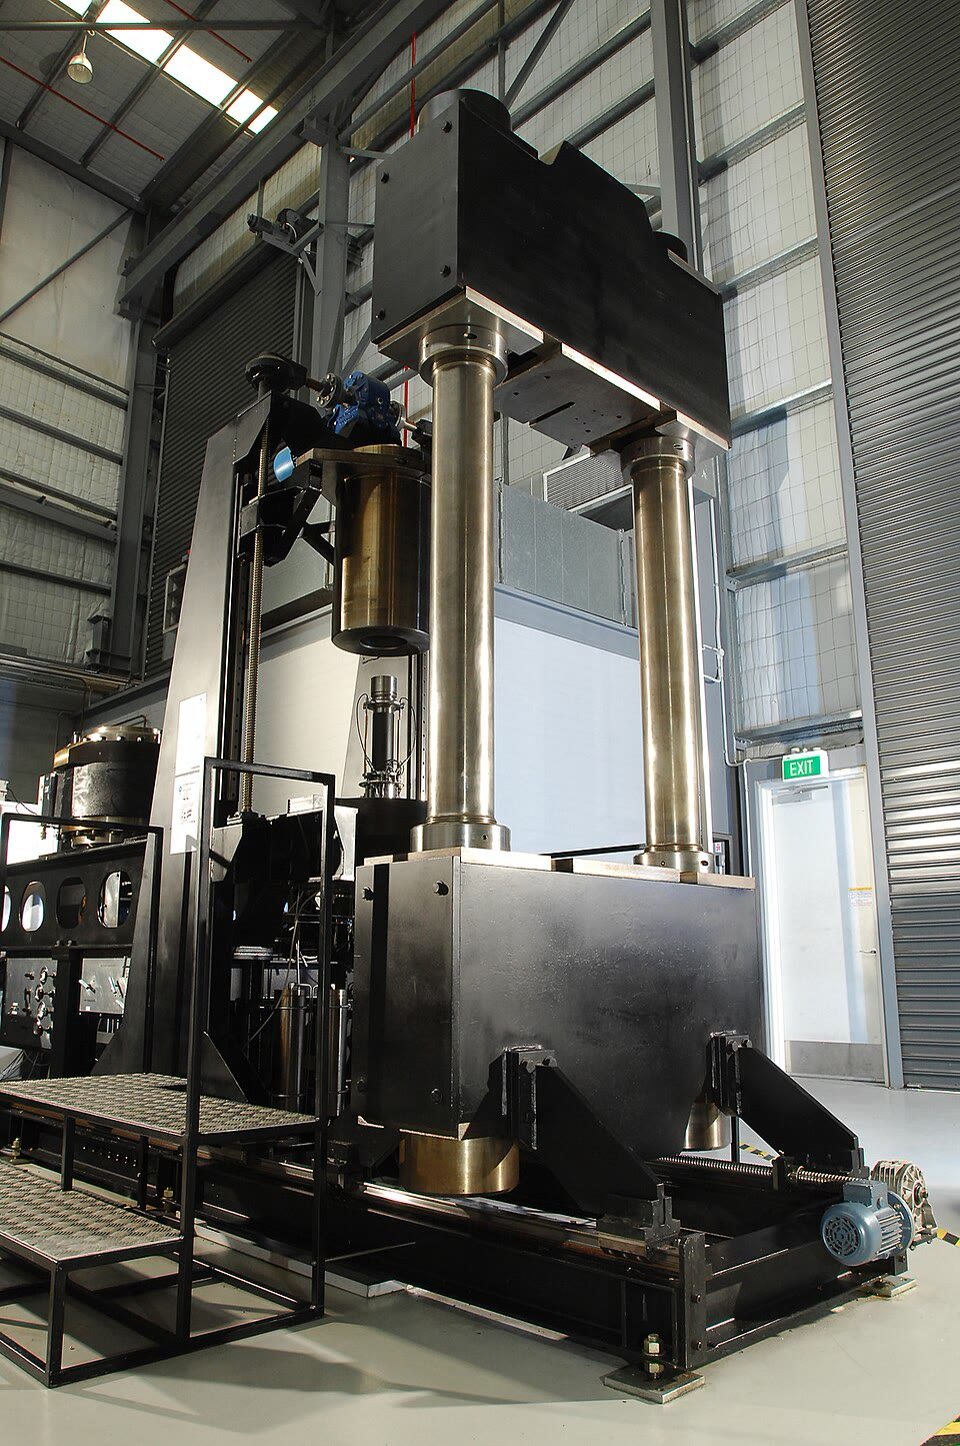
\includegraphics[width=\linewidth]{images/book3/b1-triaxial-cell.jpg}

{\scriptsize Une cellule triaxiale haute pression pour mesurer la résistance de la roche
(Darryl Peroni, CSIRO, CC BY 3.0).}
% ledger: commons:csiro-triaxial
\end{minipage}
\end{inthelab}

\section{La résistance de la lithosphère}\label{sec:b1:stress-strain-rheology:envelope}

À chaque profondeur la \omterm{def:b1:layered-earth:lithosphere}{lithosphère} peut céder de deux façons~: par glissement sur des failles,
avec une résistance qui croît avec la pression effective, ou par fluage, avec une
résistance qui diminue à mesure qu'elle chauffe. Elle se déforme de celle des deux façons qui demande la
plus petite contrainte.

\begin{definition}[Enveloppe de résistance, transition cassant--ductile, couche sismogène]\label{def:b1:stress-strain-rheology:strength-envelope}
L'\emph{enveloppe de résistance}\index{enveloppe de resistance@enveloppe de résistance} de la \omterm{def:b1:layered-earth:lithosphere}{lithosphère} est
la courbe, en fonction de la profondeur, de la plus grande \omterm{def:b1:stress-strain-rheology:principal}{contrainte différentielle} qu'elle peut supporter à une
vitesse de déformation donnée~: à chaque profondeur, la plus petite de la résistance au frottement et
de la résistance au fluage. La \emph{transition cassant--ductile}\index{transition cassant--ductile} est la profondeur où les deux sont égales~: au-dessus d'elle la roche
se déforme par failles, en dessous par fluage. La \emph{couche
sismogène}\index{couche sismogene@couche sismogène} est l'intervalle de profondeurs où commencent la plupart des
séismes.
\end{definition}

\begin{proposition}[Résistance au frottement en fonction de la profondeur]\label{prop:b1:stress-strain-rheology:brittle-gradient}
Dans une couche de masse volumique $\rho$ avec une pression interstitielle hydrostatique, une contrainte
principale verticale, des failles de toute orientation et sans \omterm{def:b1:stress-strain-rheology:coulomb}{cohésion}, le glissement avec
frottement $\mu$ commence à la \omterm{def:b1:stress-strain-rheology:principal}{contrainte différentielle}
\begin{align*}
  \sigma_1 - \sigma_3 &= \frac{2\mu}{\sqrt{1+\mu^2} + \mu}\,\rho g z(1-\lambda)
  && \text{si $\sigma_v = \sigma_1$}, \\
  \sigma_1 - \sigma_3 &= \frac{2\mu}{\sqrt{1+\mu^2} - \mu}\,\rho g z(1-\lambda)
  && \text{si $\sigma_v = \sigma_3$},
\end{align*}
avec $\lambda = \rho_w/\rho$~: le premier cas donne des failles normales, le second
des chevauchements.
\end{proposition}

\begin{proof}
La \omterm{def:b1:stress-strain-rheology:lithostatic}{contrainte effective} verticale est $S = \rho g z - \rho_w g z = \rho g z(1-\lambda)$.
Avec $C = 0$ et $k = \sqrt{1+\mu^2}$, le \cref{thm:b1:stress-strain-rheology:failure-angle}
dit qu'une faille glisse quand $r = \mu c'/k$, avec $r$ le rayon et $c'$ le
centre du cercle de Mohr effectif. Si $\sigma_v = \sigma_1$, alors
$\sigma_1' = S$ et $c' = S - r$, donc $rk = \mu S - \mu r$ et
$r = \mu S/(k+\mu)$. Si $\sigma_v = \sigma_3$, alors $c' = S + r$ et
$r = \mu S/(k-\mu)$. La \omterm{def:b1:stress-strain-rheology:principal}{contrainte différentielle} est $2r$.
\end{proof}

Avec $\mu = 0.85$ et $\rho = \qty{2700}{kg.m^{-3}}$, $S$ croît de
\qty{16.7}{MPa} par kilomètre et la résistance au frottement de
\qty{13.1}{MPa} par kilomètre en \omterm{def:b1:stress-strain-rheology:strain}{extension} et de \qty{61.3}{MPa} par
kilomètre en compression, près de cinq fois plus~: une \omterm{def:b1:layered-earth:layers}{croûte} est bien plus facile à
écarter qu'à comprimer. Au-delà d'une \omterm{def:b1:stress-strain-rheology:stress}{contrainte normale} effective de
\qty{200}{MPa} la branche supérieure de la \omterm{prop:b1:stress-strain-rheology:byerlee}{loi de Byerlee} prend le relais, et la pente
tombe, en compression, à environ \qty{35}{MPa} par kilomètre.
% computed in figdata/bachelor-1/strength_envelope.py (tested); ledger: byerlee:1975

\begin{omfigure}
\begin{tikzpicture}
\pgfplotsset{envaxis/.style={omrecord, omdepth, scale only axis, width=5.6cm, height=7.2cm,
  xmin=-1000, xmax=2500, ymin=0, ymax=80, xtick={-1000,0,1000,2000},
  ytick={0,10,...,80}, unbounded coords=jump,
  xlabel={contrainte différentielle $\sigma_1-\sigma_3$ (MPa)},
  tick label style={font=\scriptsize}, label style={font=\small},
  scaled x ticks=false, xticklabel style={/pgf/number format/.cd, 1000 sep={\,}}}}
% computed in figdata/bachelor-1/strength_envelope.py; ledger: byerlee:1975, lopez:flow-laws, codata:R, prem:moho-average
\begin{axis}[envaxis, name=cont, ylabel={profondeur (km)}, title={\small (a) continent, \qty{55}{mW.m^{-2}}}]
\addplot[fill=omLithGranite!45, draw=none] table[x=x, y=depth] {figdata/out/bachelor-1-strength_envelope-continental-outline.dat};
\addplot[omThm, line width=0.5pt, restrict x to domain=-1:2450] table[x=thrust, y=depth] {figdata/out/bachelor-1-strength_envelope-continental.dat};
\addplot[omThm, line width=0.5pt, restrict x to domain=-2450:1] table[x expr=-\thisrow{normal}, y=depth] {figdata/out/bachelor-1-strength_envelope-continental.dat};
\addplot[omDef, line width=0.5pt, restrict x to domain=-1:2450] table[x=ductile, y=depth] {figdata/out/bachelor-1-strength_envelope-continental.dat};
\addplot[omDef, line width=0.5pt, restrict x to domain=-2450:1] table[x expr=-\thisrow{ductile}, y=depth] {figdata/out/bachelor-1-strength_envelope-continental.dat};
\addplot[black, line width=1.0pt] table[x=x, y=depth] {figdata/out/bachelor-1-strength_envelope-continental-outline.dat};
\draw[black!60, dashed] (axis cs:-1000,35) -- (axis cs:2500,35);
\node[font=\scriptsize, anchor=south east] at (axis cs:2480,35) {Moho};
\draw[black, densely dotted] (axis cs:0,0) -- (axis cs:0,80);
\draw[black!70] (axis cs:660,13.7) -- (axis cs:1700,18) node[anchor=north, font=\scriptsize, align=center, text=black] {transition\\ \qty{14}{km}};
\draw[black!70] (axis cs:1870,44.6) -- (axis cs:1950,53) node[anchor=north, font=\scriptsize, align=center, text=black] {transition\\ du manteau};
\node[font=\scriptsize, anchor=north, omThm] at (axis cs:1500,3) {compression};
\node[font=\scriptsize, anchor=north, omThm] at (axis cs:-560,3) {extension};
\node[font=\scriptsize, anchor=west, omDef] at (axis cs:40,31) {quartz humide};
\node[font=\scriptsize, anchor=west, omDef] at (axis cs:300,66) {olivine sèche};
\end{axis}
\begin{axis}[envaxis, at={(cont.east)}, anchor=west, xshift=0.6cm, yticklabels={}, title={\small (b) plancher océanique de \qty{60}{\Ma}}]
\addplot[fill=omLithBasalt!45, draw=none] table[x=x, y=depth] {figdata/out/bachelor-1-strength_envelope-oceanic-outline.dat};
\addplot[omThm, line width=0.5pt, restrict x to domain=-1:2450] table[x=thrust, y=depth] {figdata/out/bachelor-1-strength_envelope-oceanic.dat};
\addplot[omThm, line width=0.5pt, restrict x to domain=-2450:1] table[x expr=-\thisrow{normal}, y=depth] {figdata/out/bachelor-1-strength_envelope-oceanic.dat};
\addplot[omDef, line width=0.5pt, restrict x to domain=-1:2450] table[x=ductile, y=depth] {figdata/out/bachelor-1-strength_envelope-oceanic.dat};
\addplot[omDef, line width=0.5pt, restrict x to domain=-2450:1] table[x expr=-\thisrow{ductile}, y=depth] {figdata/out/bachelor-1-strength_envelope-oceanic.dat};
\addplot[black, line width=1.0pt] table[x=x, y=depth] {figdata/out/bachelor-1-strength_envelope-oceanic-outline.dat};
\draw[black, densely dotted] (axis cs:0,0) -- (axis cs:0,80);
\draw[black!70] (axis cs:2003,38.2) -- (axis cs:1900,50) node[anchor=north, font=\scriptsize, align=center, text=black] {transition\\ \qty{38}{km}};
\node[font=\scriptsize, anchor=west, omDef] at (axis cs:300,66) {olivine sèche};
\end{axis}
\end{tikzpicture}
\par\smallskip{\small \omterm{def:b1:stress-strain-rheology:strength-envelope}{Enveloppes de résistance} à la vitesse de déformation
\qty{e-15}{s^{-1}}. Rouge~: résistance au frottement d'après la \omterm{prop:b1:stress-strain-rheology:byerlee}{loi de Byerlee} avec une
pression interstitielle hydrostatique, pour la compression (failles inverses, à droite) et
l'\omterm{def:b1:stress-strain-rheology:strain}{extension} (failles normales, à gauche, tracées en négatif)~; bleu~: la résistance au fluage
de la quartzite humide dans la \omterm{def:b1:layered-earth:layers}{croûte} continentale et de l'\omterm{def:b1:rock-forming-minerals:groups}{olivine} sèche dans le \omterm{def:b1:layered-earth:layers}{manteau}~;
contour noir et grisé~: la résistance, la plus petite des deux à chaque
profondeur. (a) Un continent de flux de chaleur de surface \qty{55}{mW.m^{-2}} et de
\omterm{def:b1:layered-earth:layers}{croûte} épaisse de \qty{35}{km}~: \omterm{def:b1:layered-earth:layers}{croûte} supérieure forte, \omterm{def:b1:layered-earth:layers}{croûte} inférieure faible, tout
haut du \omterm{def:b1:layered-earth:layers}{manteau} fort. (b) Plancher océanique de \qty{60}{\Ma}~: une seule couche forte,
épaisse de \qty{38}{km} en compression.}
\label{fig:b1:stress-strain-rheology:envelope}
\end{omfigure}

La figure ci-dessus met les deux résistances ensemble
pour deux \omterm{def:b1:layered-earth:lithosphere}{lithosphères}. Le continent a le \omterm{def:b1:heat-budget:geotherm}{géotherme} du
\cref{ch:b1:heat-budget} avec un flux de chaleur de surface de \qty{55}{mW.m^{-2}}, une
\omterm{def:b1:layered-earth:layers}{croûte} de quartzite humide épaisse de \qty{35}{km}, et de l'\omterm{def:b1:rock-forming-minerals:groups}{olivine} sèche en dessous~; le plancher
océanique a \qty{60}{\Ma}, avec le \omterm{def:b1:heat-budget:geotherm}{géotherme} du demi-espace du même chapitre,
et de l'\omterm{def:b1:rock-forming-minerals:groups}{olivine} du fond marin vers le bas. La vitesse de déformation est
\qty{e-15}{s^{-1}}. Les \qty{35}{km} sont la profondeur moyenne du \omterm{def:b1:layered-earth:discontinuity}{Moho} sous
les continents dans le \omterm{def:b1:layered-earth:reference-model}{modèle de Terre de référence} du \cref{ch:b1:layered-earth}.
% ledger: prem:moho-average

Sous le continent la \omterm{def:b1:stress-strain-rheology:strength-envelope}{transition cassant--ductile} tombe à \qty{13.7}{km}
en compression, à \qty{249}{\degreeCelsius}, et à \qty{17.1}{km} en
\omterm{def:b1:stress-strain-rheology:strain}{extension}. Une \omterm{def:b1:layered-earth:layers}{croûte} plus chaude la ferait remonter, une plus froide l'enfoncerait,
puisque la loi de fluage ne dépend que de la température à une contrainte donnée. La
transition est le niveau le plus résistant de la \omterm{def:b1:layered-earth:layers}{croûte}.
En dessous la résistance s'effondre~: au \omterm{def:b1:layered-earth:discontinuity}{Moho}, à \qty{527}{\degreeCelsius},
la quartzite s'écoule sous \qty{7.6}{MPa}, alors que l'\omterm{def:b1:rock-forming-minerals:groups}{olivine} à la même température
demanderait quelque \qty{30000}{MPa}, si loin au-delà de la résistance au frottement que
le haut du \omterm{def:b1:layered-earth:layers}{manteau} est de nouveau cassant. Une seconde transition suit à
\qty{44.6}{km} en compression. La \omterm{def:b1:layered-earth:layers}{croûte} inférieure de ce modèle est une couche molle
entre deux couches fortes~: le «~sandwich à la gelée~». Sous l'océan toute la
\omterm{def:b1:layered-earth:lithosphere}{lithosphère} est de l'\omterm{def:b1:rock-forming-minerals:groups}{olivine}, et la résistance croît jusqu'à une seule transition à
\qty{38.2}{km}, à \qty{641}{\degreeCelsius}.
% computed in figdata/bachelor-1/strength_envelope.py (tested)

Les séismes s'accordent avec l'enveloppe océanique~: à l'intérieur des plaques océaniques,
ils atteignent des profondeurs où la température est de
\qtyrange{600}{800}{\degreeCelsius}, proche des \qty{641}{\degreeCelsius}
de la transition unique du modèle. Des séismes plus profonds ne se produisent que là où une
plaque plonge sous une autre, jusqu'à plus de \qty{700}{km}
(\cref{ch:b1:active-margins}).
% ledger: jackson:jelly, usgs:deepest

Le \omterm{def:b1:layered-earth:layers}{manteau} continental est là où le tableau est contesté. Pendant une vingtaine
d'années le sandwich à la gelée a été l'opinion dominante, bâtie sur des mesures de laboratoire
sur l'\omterm{def:b1:rock-forming-minerals:groups}{olivine} sèche et sur quelques séismes que l'on croyait situés sous
le \omterm{def:b1:layered-earth:discontinuity}{Moho}. En 2002 James Jackson a soutenu qu'il fallait l'abandonner~: de meilleures
profondeurs montraient que les séismes dans les continents sont confinés à une seule
couche, d'ordinaire la \omterm{def:b1:layered-earth:layers}{croûte} supérieure, parfois toute la \omterm{def:b1:layered-earth:layers}{croûte}, sans séismes
convaincants dans le \omterm{def:b1:layered-earth:layers}{manteau} en dessous, même là où le \omterm{def:b1:layered-earth:discontinuity}{Moho} n'est qu'à
\qtyrange{300}{500}{\degreeCelsius}. De petites quantités d'eau, quelques parties par
million dans l'\omterm{def:b1:rock-forming-minerals:groups}{olivine}, suffisent à l'affaiblir considérablement, et le \omterm{def:b1:layered-earth:layers}{manteau}
continental pourrait fort bien en contenir autant~; la résistance des continents résiderait alors
surtout dans leur \omterm{def:b1:layered-earth:layers}{croûte}. Les deux visions tracent des enveloppes différentes à partir des mêmes
lois, avec de l'\omterm{def:b1:rock-forming-minerals:groups}{olivine} sèche ou humide sous le \omterm{def:b1:layered-earth:discontinuity}{Moho}.
% ledger: jackson:jelly
Quelle que soit la bonne, une enveloppe est une borne et non une mesure~: les
lois de laboratoire sont extrapolées sur de nombreux ordres de grandeur de vitesse de déformation,
et les contraintes maximales qu'elle montre, plus d'un gigapascal, sont bien au-dessus des
\qtyrange{1}{10}{MPa} que l'on voit libérés par les séismes.
% ledger: jackson:jelly

\section{Exercices}

\begin{exercise}[$\star$]\label{exo:b1:stress-strain-rheology:1}
Prendre une \omterm{def:b1:layered-earth:layers}{croûte} de masse volumique \qty{2700}{kg.m^{-3}} et $g = \qty{9.81}{m.s^{-2}}$.
À une profondeur de \qty{10}{km}, calculer (a) la contrainte verticale, (b) la
pression interstitielle hydrostatique, (c) la \omterm{def:b1:stress-strain-rheology:lithostatic}{contrainte effective} verticale et le
rapport de pression interstitielle $\lambda$.
\end{exercise}

\begin{exercise}[$\star$]\label{exo:b1:stress-strain-rheology:2}
(a) Un banc de \qty{10}{km} de long est étiré jusqu'à \qty{13}{km}~: donner son \omterm{def:b1:stress-strain-rheology:strain}{extension}
et son \omterm{def:b1:stress-strain-rheology:strain}{étirement}. (b) Un autre, de \qty{10}{km} de long, est raccourci jusqu'à \qty{7}{km}.
(c) Deux lignes d'une roche qui étaient perpendiculaires font maintenant un angle de
\ang{60}~: quels sont le cisaillement angulaire et la \omterm{def:b1:stress-strain-rheology:strain}{déformation de cisaillement}~?
\end{exercise}

\begin{exercise}[$\star$]\label{exo:b1:stress-strain-rheology:3}
En un point, $\sigma_1 = \qty{100}{MPa}$ et $\sigma_3 = \qty{40}{MPa}$.
(a) Tracer le cercle de Mohr. (b) Quelle est la plus grande contrainte de cisaillement, sur quels
plans agit-elle, et quelle \omterm{def:b1:stress-strain-rheology:stress}{contrainte normale} agit sur eux~? (c) Calculer $\sigma_n$
et $\tau$ sur le plan dont la normale fait \ang{30} avec $\sigma_1$.
\end{exercise}

\begin{exercise}[$\star$]\label{exo:b1:stress-strain-rheology:4}
Une roche a la \omterm{def:b1:stress-strain-rheology:coulomb}{cohésion} \qty{10}{MPa} et l'\omterm{def:b1:stress-strain-rheology:coulomb}{angle de frottement interne}
\ang{30}. (a) Sous quel angle avec $\sigma_1$ se rompt-elle, et quel angle les
deux plans de fracture possibles font-ils entre eux~? (b) Avec
$\sigma_3' = \qty{20}{MPa}$, quelle $\sigma_1'$ effective la rompt~?
\end{exercise}

\begin{exercise}[$\star\star$]\label{exo:b1:stress-strain-rheology:5}
Dans les axes $x$ (horizontal) et $y$ (vertical), $\sigma_{xx} = \qty{60}{MPa}$,
$\sigma_{yy} = \qty{20}{MPa}$ et $\sigma_{xy} = \qty{15}{MPa}$. (a) Calculer les
\omterm{def:b1:stress-strain-rheology:principal}{contraintes principales} et l'angle $\theta_p$. (b) Vérifier avec la
\cref{prop:b1:stress-strain-rheology:transformation} que le plan de normale
$\theta_p$ ne porte aucune contrainte de cisaillement et porte la \omterm{def:b1:stress-strain-rheology:stress}{contrainte normale} $\sigma_1$. (c) Quelle est
la plus grande contrainte de cisaillement en ce point~?
\end{exercise}

\begin{exercise}[$\star\star$]\label{exo:b1:stress-strain-rheology:6}
Une zone de cisaillement a déformé sa roche par un \omterm{def:b1:stress-strain-rheology:shear-types}{cisaillement simple} $\gamma = 2$. (a) Calculer
les \omterm{def:b1:stress-strain-rheology:strain}{étirements} principaux et l'angle du grand axe de l'\omterm{def:b1:stress-strain-rheology:strain-ellipse}{ellipse de déformation}
avec la direction de cisaillement. (b) Vérifier que l'aire n'a pas changé. (c) Une ligne de
matière était à \ang{45} de la direction de cisaillement, montant dans le sens du
cisaillement~: où se trouve-t-elle maintenant, et quel est son \omterm{def:b1:stress-strain-rheology:strain}{étirement}~? Comparer avec (a).
\end{exercise}

\begin{exercise}[$\star\star$]\label{exo:b1:stress-strain-rheology:7}
Dans une zone de cisaillement épaisse de \qty{200}{m}, de petites taches rondes dans une ardoise sont devenues des
ellipses d'axes dans le rapport de 4 à 1. Supposer un \omterm{def:b1:stress-strain-rheology:shear-types}{cisaillement simple}, sans changement
d'aire. (a) Trouver $S_1$, $S_2$ et $\gamma$. (b) Sous quel angle avec les parois de
la zone les grands axes devraient-ils se coucher~? (c) De quelle distance une paroi a-t-elle glissé le long de
l'autre~?
\end{exercise}

\begin{exercise}[$\star\star$]\label{exo:b1:stress-strain-rheology:8}
Une faille à une profondeur de \qty{3}{km}, dans une \omterm{def:b1:layered-earth:layers}{croûte} de masse volumique \qty{2700}{kg.m^{-3}},
porte la \omterm{def:b1:stress-strain-rheology:stress}{contrainte normale} \qty{70}{MPa} et la contrainte de cisaillement \qty{30}{MPa}.
(a) Avec une pression interstitielle hydrostatique, glisse-t-elle d'après la \omterm{prop:b1:stress-strain-rheology:byerlee}{loi de Byerlee}~?
(b) Et si les pores sont scellés et $\lambda = 0.6$~? (c) Trouver la valeur
de $\lambda$ à laquelle elle commence à glisser.
\end{exercise}

\begin{exercise}[$\star\star$]\label{exo:b1:stress-strain-rheology:9}
Utiliser la loi de fluage de la quartzite humide (\cref{prop:b1:stress-strain-rheology:creep}).
(a) De quel facteur la contrainte doit-elle croître pour qu'elle s'écoule dix fois plus vite~?
(b) De quel facteur sa résistance chute-t-elle entre \qty{400}{\degreeCelsius}
et \qty{500}{\degreeCelsius}, à la même vitesse et avec $V = 0$~? (c) Expliquer
avec ces deux résultats pourquoi la profondeur de la \omterm{def:b1:stress-strain-rheology:strength-envelope}{transition cassant--ductile}
dépend bien plus du \omterm{def:b1:heat-budget:geotherm}{géotherme} que de la vitesse de déformation.
\end{exercise}

\begin{exercise}[$\star\star\star$]\label{exo:b1:stress-strain-rheology:10}
Là où la contrainte verticale est $\sigma_2$, les failles sont décrochantes. Supposer que
la \omterm{def:b1:stress-strain-rheology:lithostatic}{contrainte effective} verticale est alors la moyenne $(\sigma_1' + \sigma_3')/2$.
(a) Montrer que le glissement avec frottement $\mu$ et sans \omterm{def:b1:stress-strain-rheology:coulomb}{cohésion} commence à
$\sigma_1 - \sigma_3 = 2\mu\,\rho g z(1-\lambda)/\sqrt{1+\mu^2}$. (b) Calculer
la pente en mégapascals par kilomètre pour $\mu = 0.85$ et
$\rho = \qty{2700}{kg.m^{-3}}$, et la placer entre les pentes des failles normales et
inverses. (c) Exprimer chacune des trois pentes comme un multiple de la
\omterm{def:b1:stress-strain-rheology:lithostatic}{contrainte effective} verticale.
\end{exercise}

\begin{exercise}[$\star\star\star$]\label{exo:b1:stress-strain-rheology:11}
Modéliser la \omterm{def:b1:layered-earth:lithosphere}{lithosphère} océanique de \qty{60}{\Ma} comme un demi-espace refroidi depuis
\qty{1350}{\degreeCelsius}, avec une surface à \qty{0}{\degreeCelsius} et
$\kappa = \qty{e-6}{m^2.s^{-1}}$~: $T = \num{1350}\operatorname{erf}\bigl(z/(2\sqrt{\kappa t})\bigr)$.
(a) Calculer $2\sqrt{\kappa t}$. (b) Trouver les profondeurs des isothermes
\qty{600}{\degreeCelsius} et \qty{800}{\degreeCelsius}. (c) Les séismes
à l'intérieur des plaques océaniques atteignent les profondeurs où la température est de
\qtyrange{600}{800}{\degreeCelsius}. Comparer avec la \omterm{def:b1:stress-strain-rheology:strength-envelope}{transition cassant--ductile} de
l'\omterm{def:b1:stress-strain-rheology:strength-envelope}{enveloppe de résistance} océanique de ce chapitre, à
\qty{38.2}{km} et \qty{641}{\degreeCelsius}.
% ledger: jackson:jelly
\end{exercise}

\begin{exercise}[$\star\star\star$]\label{exo:b1:stress-strain-rheology:12}
Une roche est traversée de fractures de toute orientation, toutes contenant la
direction de $\sigma_2$, sans \omterm{def:b1:stress-strain-rheology:coulomb}{cohésion} et de frottement 0.85. Les \omterm{def:b1:stress-strain-rheology:principal}{contraintes principales}
effectives sont $\sigma_1' = \qty{110}{MPa}$ et
$\sigma_3' = \qty{20}{MPa}$. (a) Montrer que certaines fractures glissent. (b) Trouver
l'intervalle de l'angle entre les fractures qui glissent et $\sigma_1$. Laquelle est
au milieu de l'intervalle~? (c) Jusqu'à quelle valeur de $\sigma_1'$, avec
$\sigma_3'$ fixée, au moins une fracture glisse-t-elle encore~?
\end{exercise}

\section{Problème~: La faille va-t-elle glisser~?}

\begin{problem}[{Problème du week-end --- la contrainte sur une faille normale à une profondeur
de cinq kilomètres, sa marge de sécurité, et la hausse de pression interstitielle qui
la ferait glisser}]
\label{pb:b1:stress-strain-rheology:1}
% values: calc/ch16.py; ledger: byerlee:1975, hb81:denver
Une faille est orientée nord--sud et plonge de \ang{60} vers l'est. Un puits d'élimination
l'atteint à une profondeur de \qty{5.00}{km}, dans une \omterm{def:b1:layered-earth:layers}{croûte} de masse volumique
\qty{2700}{kg.m^{-3}} dont les pores communiquent avec la surface. Une mesure dans le
puits donne la contrainte horizontale perpendiculaire à la faille,
\qty{75.0}{MPa}~; la contrainte horizontale selon la direction se situe entre elle et
la contrainte verticale, si bien que le problème est à deux dimensions dans le plan vertical
est--ouest. Prendre $g = \qty{9.81}{m.s^{-2}}$, l'eau de masse volumique
\qty{1000}{kg.m^{-3}} et la \omterm{prop:b1:stress-strain-rheology:byerlee}{loi de Byerlee}. Donner les contraintes à
\qty{0.01}{MPa}.

\medskip
\noindent\textbf{Partie I --- L'état de contrainte.}
\begin{enumerate}
  \item Calculer la contrainte verticale à la profondeur de la faille.
  \item Calculer la pression interstitielle hydrostatique en ce lieu, et le rapport $\lambda$.
  \item Laquelle des deux contraintes est $\sigma_1$ et laquelle $\sigma_3$~? Quelle sorte
        de faille cet état de contrainte entraîne-t-il~?
  \item Calculer la \omterm{def:b1:stress-strain-rheology:principal}{contrainte différentielle}, le centre et le rayon du
        cercle de Mohr.
  \item Calculer les \omterm{def:b1:stress-strain-rheology:principal}{contraintes principales} effectives et le centre du
        cercle effectif.
  \item Avec $x$ horizontal vers l'est et $y$ vertical, écrire les trois
        composantes $\sigma_{xx}$, $\sigma_{yy}$, $\sigma_{xy}$. Pourquoi
        $\sigma_{xy}$ est-elle nulle~?
\end{enumerate}

\medskip
\noindent\textbf{Partie II --- Les contraintes sur la faille.}
\begin{enumerate}[resume]
  \item Donner la normale unitaire à la faille dans les axes de la question 6, et
        l'angle $\theta$ entre elle et $\sigma_1$.
  \item Calculer $\sigma_n$ et $\tau$ sur la faille avec
        la \cref{prop:b1:stress-strain-rheology:transformation}.
  \item Vérifier les deux valeurs avec le cercle de Mohr~: sous quel angle depuis l'extrémité
        $\sigma_1$ se trouve la faille~?
  \item Calculer la \omterm{def:b1:stress-strain-rheology:stress}{contrainte normale} effective sur la faille.
  \item Calculer le rapport $\tau/\sigma_n'$ et le comparer à 0.85.
  \item Quelle contrainte de cisaillement ferait glisser la faille sous la \omterm{def:b1:stress-strain-rheology:stress}{contrainte
        normale} effective actuelle~? De combien de mégapascals en est-elle éloignée~?
\end{enumerate}

\medskip
\noindent\textbf{Partie III --- Le cercle de Mohr et la loi de Byerlee.}
\begin{enumerate}[resume]
  \item Tracer le cercle de Mohr effectif et la droite de Byerlee à l'échelle.
  \item Calculer la distance du centre du cercle à la droite et la
        comparer au rayon. Un plan quelconque de la roche peut-il glisser~?
  \item Quel plan glisserait le premier~? Donner son angle avec $\sigma_1$ et son \omterm{def:b1:geological-maps:attitude}{pendage}.
  \item Avec la \cref{prop:b1:stress-strain-rheology:brittle-gradient}, calculer la
        \omterm{def:b1:stress-strain-rheology:principal}{contrainte différentielle} à laquelle les failles normales glissent à cette profondeur, et
        la vérifier avec la pente de \qty{13.1}{MPa} par kilomètre.
  \item À quel niveau la contrainte horizontale devrait-elle tomber pour que le plan le mieux
        orienté glisse~?
  \item À quel niveau pour que la faille du problème glisse~? Expliquer pourquoi il est
        plus bas.
\end{enumerate}

\medskip
\noindent\textbf{Partie IV --- L'injection.}
\begin{enumerate}[resume]
  \item Expliquer pourquoi une hausse $\Delta P$ de la pression interstitielle déplace le cercle
        effectif de $\Delta P$ vers la gauche sans changer son rayon.
  \item Calculer la hausse de pression interstitielle qui amène le plan le mieux orienté
        à glisser.
  \item Le puits est plein d'eau. Quelle pression supplémentaire la pompe doit-elle appliquer
        en tête de puits pour élever la pression interstitielle à la faille de cette quantité~?
        À quelle hauteur de colonne d'eau cela équivaut-il~?
  \item Si le frottement sur la faille était de 0.6 plutôt que 0.85, glisserait-elle
        déjà~? Que dit le calme de la faille de son
        frottement~?
  \item À quel rapport $\lambda$ le plan le mieux orienté glisse-t-il~?
  \item À une décimale, en mégapascals, quelle hausse de pression interstitielle amène cette
        faille à glisser~?
\end{enumerate}
\end{problem}
